\documentclass[12pt,xcolor=dvipsnames]{article}
\usepackage[utf8]{inputenc}
\usepackage[vietnamese]{babel}
\usepackage{amstext,latexsym,amsbsy,amssymb,amsmath,amsthm,amsfonts,exscale,eucal}
\usepackage{appendix}
\usepackage{algorithm}
\usepackage{graphicx}
\usepackage{xcolor}
\usepackage{hyperref}
\usepackage{indentfirst}
\usepackage{enumitem}
\usepackage{diagbox}

\usepackage[left=2.00cm, right=2.00cm, top=2.00cm, bottom=2.00cm]{geometry}
\setlength{\parskip}{5pt}%khoảng cách dòng
\renewcommand{\baselinestretch}{1.15}
\theoremstyle{definition}
\newtheorem{vd}{Ví dụ}[section]
\newtheorem*{giai}{Giải}
\newtheorem{bt}{Bài tập}
\renewcommand{\l}{\left}
\renewcommand{\r}{\right}
\date{}

\begin{document}
\begin{bt}
Thực hiện các bài toán mô phỏng sau:
\begin{enumerate}
    \item[(a)] Sử dụng bài toán ước lượng trung bình của phân phối Cauchy chuẩn để minh họa cách phương pháp bootstrap có thể thất bại đối với các phân phối có đuôi nặng.
    \item[(b)] Sử dụng bài toán ước lượng $\theta$ cho phân phối $U(0, \theta)$ để minh họa cách phương pháp bootstrap có thể thất bại đối với các giá trị cực trị.
\end{enumerate}
\end{bt}

\begin{giai}
\textbf{1. Phân phối Cauchy (Đuôi nặng)}

Phân phối Cauchy chuẩn có hàm mật độ xác suất $f(x) = \frac{1}{\pi(1+x^2)}$. Đặc điểm nổi bật của phân phối này là kỳ vọng và phương sai không xác định (đuôi rất nặng).

\textit{Chứng minh phương sai không hữu hạn:}
Xét moment bậc hai $E[X^2]$:
\[
E[X^2] = \int_{-\infty}^{\infty} \frac{x^2}{\pi(1+x^2)} dx = \frac{1}{\pi} \int_{-\infty}^{\infty} \left(1 - \frac{1}{1+x^2}\right) dx
\]
\[
= \frac{1}{\pi} \left[ x - \arctan(x) \right]_{-\infty}^{\infty} = \infty
\]
Do tích phân phân kỳ, $E[X^2]$ không tồn tại hữu hạn, dẫn đến phương sai không xác định.

Theo lý thuyết giới hạn trung tâm,
 nếu phương sai hữu hạn, trung bình mẫu sẽ hội tụ về phân phối chuẩn. 
 Tuy nhiên, với Cauchy, trung bình mẫu cũng tuân theo phân phối Cauchy và không bao giờ hội 
 tụ về một giá trị duy nhất khi $n \to \infty$. Do đó, phân phối bootstrap của trung bình mẫu
  sẽ rất bất ổn định (erratic), có độ phân tán cực lớn và không phản ánh đúng tính chất hội tụ.

\begin{center}
    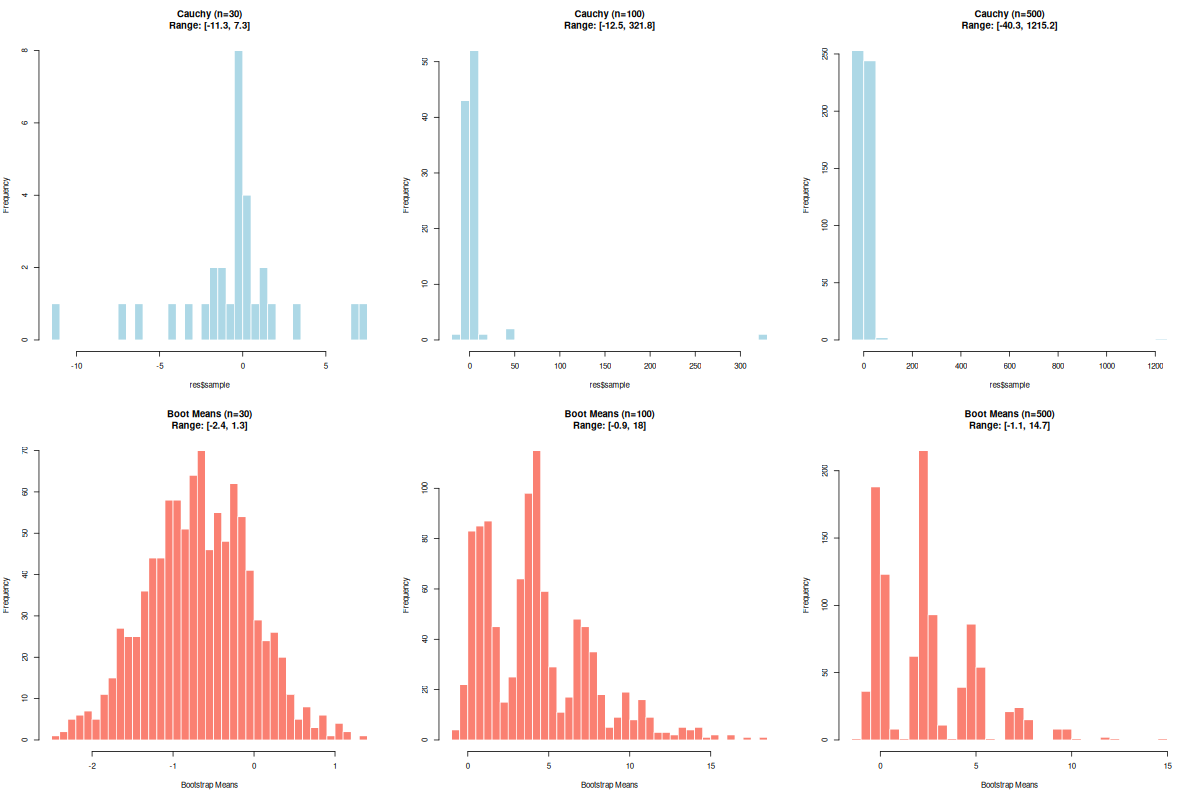
\includegraphics[width=0.8\textwidth]{cauchy_bootstrap_failure_varying_n.png}
\end{center}

Hình trên minh họa:
\begin{itemize}
    \item Mẫu gốc có thể chứa các giá trị ngoại lai rất lớn (do đuôi nặng).
    \item Phân phối bootstrap của trung bình mẫu (`Bootstrap Distribution of Mean`) không có hình dạng chuông ổn định mà dẹt và lan rộng, hoặc phụ thuộc rất nhiều vào các giá trị ngoại lai cụ thể trong mẫu gốc. Khoảng tin cậy bootstrap sẽ cực kỳ rộng và không đáng tin cậy.
\end{itemize}

\textbf{2. Phân phối Đều $U(0, \theta)$ (Biên cực trị)}

Xét bài toán ước lượng tham số $\theta$ dựa trên ước lượng 
hợp lý cực đại $\hat{\theta} = \max(X_1, \ldots, X_n)$.

Phân phối thực của $n(\theta - \hat{\theta})$ hội tụ về phân phối mũ (Exponential distribution). 
Tuy nhiên, phương pháp naive bootstrap thất bại trong trường hợp này. 
Lý do là giá trị lớn nhất của mẫu bootstrap, $\theta^* = \max(X^*)$, không bao giờ vượt quá $\hat{\theta}$ của mẫu gốc.

\begin{equation}
P(\theta^* = \hat{\theta}) = 1 - (1 - 1/n)^n \approx 1 - e^{-1} \approx 0.632
\end{equation}

Tức là trong khoảng 63.2\% số lần lặp bootstrap, giá trị ước lượng bootstrap sẽ đúng bằng $\hat{\theta}$. Điều này tạo ra một phân phối rời rạc, co cụm tại $\hat{\theta}$, khác xa với phân phối liên tục thực tế của ước lượng.

\begin{center}
    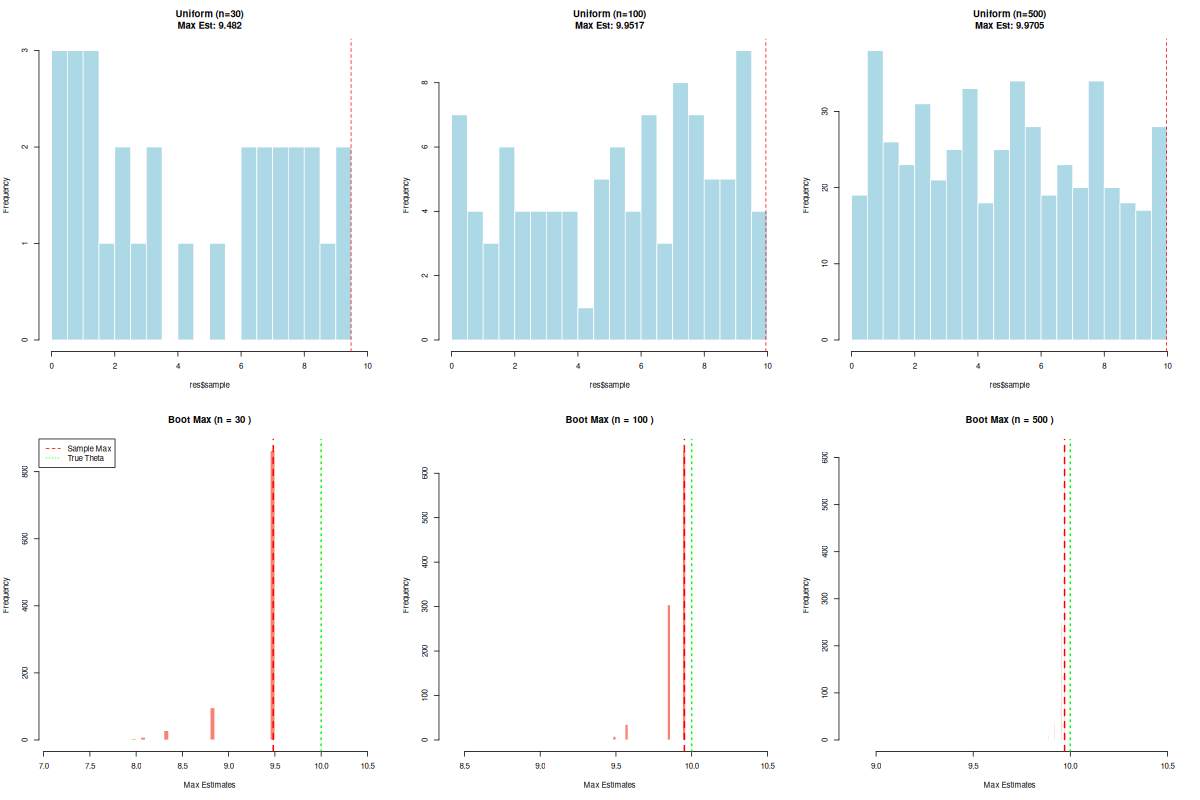
\includegraphics[width=0.8\textwidth]{uniform_bootstrap_failure_varying_n.png}
\end{center}

Hình trên minh họa:
\begin{itemize}
    \item Phân phối bootstrap tập trung xác suất lớn tại giá trị $\hat{\theta}$ (cực đại của mẫu gốc).
    \item Nó không mô phỏng được hành vi của $\hat{\theta}$ đối với tham số thực $\theta$ (vốn luôn lớn hơn hoặc bằng $\hat{\theta}$), dẫn đến ước lượng khoảng tin cậy bị sai lệch (phủ không đúng).
\end{itemize}

\textbf{3. Mã nguồn}

Mã nguồn R thực hiện mô phỏng được lưu tại \texttt{exercise\_03.R}.

\end{giai}
\end{document}
